% !TeX encoding = UTF-8
% Do not touch the below 70 lines
\documentclass[11pt, a4paper, onecolumn, oneside]{report}

\usepackage{mathptmx}
\usepackage[T1]{fontenc}
\usepackage[utf8]{inputenc}

\RequirePackage[top=3cm, bottom=1in, left=1in, right=1in]{geometry}
\linespread{1.3}

\usepackage{titlesec}
\usepackage{amsmath}
\usepackage{amssymb}
\usepackage{mathtools}
\usepackage{enumerate}
\usepackage{bbm}
\usepackage{algorithm}
\usepackage{algorithmic}
\usepackage{epsfig}
\usepackage{color}
\usepackage{graphicx}
\usepackage{caption}
\usepackage{subcaption}
\usepackage{cases}
\usepackage{url}
\usepackage{cite}
\usepackage{fancyhdr}
\usepackage{tocloft}
\usepackage{pdfpages}

\usepackage{acro}
\usepackage[notocbib]{apacite}
\usepackage{kotex}
\usepackage{microtype}
\setcounter{secnumdepth}{5}
\setcounter{tocdepth}{5}

\DeclareAcronym{ptb}
{
    short=PTB,
    long=Preterm birth
}

\DeclareAcronym{rrna}
{
    short=rRNA,
    long=Ribosomal RNA
}

\DeclareAcronym{ftb}
{
    short=FTB,
    long=Full-term birth
}

\DeclareAcronym{dat}
{
    short=DAT,
    long=Differentially abundant taxa
}

\DeclareAcronym{prom}
{
    short=PROM,
    long=Prelabor rupture of membrane
}

\DeclareAcronym{ga}
{
    short=GA,
    long=Gestational age
}

\DeclareAcronym{acc}
{
    short=ACC,
    long=Accuracy
}

\DeclareAcronym{ba}
{
    short=BA,
    long=Balanced accuracy
}

\DeclareAcronym{sen}
{
    short=SEN,
    long=Sensitivity
}

\DeclareAcronym{spe}
{
    short=SPE,
    long=specificity
}

\DeclareAcronym{pre}
{
    short=PRE,
    long=Precision
}

\DeclareAcronym{asv}
{
    short=ASV,
    long=Amplicon sequence variant
}

\DeclareAcronym{faithpd}
{
    short=Faith PD,
    long=Faith's phylogenetic diversity
}



\renewcommand\cftsecafterpnum{\vskip15pt}
\renewcommand\cftsubsecafterpnum{\vskip15pt}
\renewcommand\cftfigafterpnum{\vskip15pt}
\renewcommand{\thesection}{\arabic{section}}
\renewcommand{\thesubsection}{\arabic{section}.\arabic{subsection}}
\renewcommand{\thesubsubsection}{\arabic{section}.\arabic{subsection}.\arabic{subsubsection}}
\renewcommand{\contentsname}{\hfill\bfseries\Large Contents\hfill}
\renewcommand{\listfigurename}{\hfill\bfseries\Large List of Figures\hfill}
\renewcommand{\listtablename}{\hfill\bfseries\Large List of Tables\hfill}
\renewcommand{\thefigure}{\arabic{figure}}
\newcommand{\qed}{\hfill\blacksquare}
\renewcommand{\bibname}{\hfill\bfseries\Large References \hfill\hfill}
\renewcommand{\abstractname}{\bfseries\Large Abstract \hfill\hfill}

\newcounter{lemma}
\newcounter{proposition}
\newcounter{theorem}
\newtheorem{lemma}{\bf Lemma}
\newtheorem{proposition}{\bf Proposition}
\newtheorem{theorem}{\bf Theorem}
\newtheorem{proof}{\bf Proof}

\newcommand{\HIGH}[1]{{\textcolor{blue}{#1}}}
%\renewcommand{\baselinestretch}{1.5}

\DeclareMathOperator*{\argmax}{arg\,max}

\fancyhf{}
\renewcommand{\headrulewidth}{0pt}
\cfoot{\thepage}
\pagestyle{fancy}
%\pagenumbering{gobble}

% Do not touch the above 70 lines

\begin{document}
% Front cover
    \begin{center}
    \LARGE Doctoral Thesis

    \vspace{3cm}
    \huge \input{Documents/Title.txt}

    \vfill

    \LARGE \input{Documents/Name.txt}

    \vspace{2cm}

    \LARGE \input{Documents/Department.txt}

    \vspace{2cm}

    \LARGE \input{Documents/UNIST.txt}
    \vspace{2cm}

    \LARGE \the\year{}

    \end{center}
    \thispagestyle{empty}
    \clearpage

% Title page
    \begin{center}
    \hbox{ }

    \hbox{ }

    \huge \input{Documents/Title.txt}

    \vspace{5cm}

    \LARGE \input{Documents/Name.txt}

    \vspace{6cm}

    \LARGE \input{Documents/Department.txt}

    \vspace{2cm}

    \LARGE \input{Documents/UNIST.txt}

    \end{center}
    \thispagestyle{empty}
    \clearpage

% Thesis approval
% Add the approval doc signed by your advisor in a PDF file
% Put your pdf with the filename below, and uncomment it.
\includepdf[fitpaper= true, pages=-]{Documents/example.pdf}

% [Confirmation of thesis approval]
% add the certificate signed by your committee in a PDF file
% Put your pdf with the filename below, and uncomment it.
\includepdf[fitpaper= true, pages=-]{Documents/example.pdf}

% Abstract
    \begin{abstract}
        The microbiome refers to the complex community of microorganisms, including bacteria, viruses, fungi, and other microbes, that inhabit various environment within living organisms \cite{microbiome-1, microbiome-3}. In humans, the microbiome plays a crucial role in maintaining health \cite{microbiome-2}, influencing processes such as digestion \cite{microbiome-digestion-1}, immune response \cite{microbiome-immune-1, microbiome-immune-2, microbiome-immune-3}, and even mental health \cite{microbiome-mental-1, microbiome-mental-2, microbiome-mental-3}. These microbial communities are not static nor constant, but rather dynamic ecosystem that interacts with their host and respond to environmental changes. Recent studies have revealed that imbalances in the microbiome, known as dysbiosis, can contribute to a wide range of diseases, including obesity \cite{microbiome-obesity-1, microbiome-obesity-2, microbiome-obesity-3}, diabetes \cite{microbiome-diabetes-1, microbiome-diabetes-2, microbiome-diabetes-3}, infections \cite{microbiome-infection-1, microbiome-infection-2}, inflammatory conditions \cite{microbiome-inflammation-1, microbiome-inflammation-2, microbiome-inflammation-3}, and cancers \cite{microbiome-cancer-1, microbiome-cancer-2, microbiome-cancer-3, microbiome-cancer-4}. Thus, understanding the composition of the human microbiomes is essential for developing new therapeutic approaches that target these microbial populations to promote health and prevent diseases.

        (PTB)

        (Periodontitis)

        (Lung)

        (Conclusion)

        \vfill
        \noindent\rule{\linewidth}{0.4pt}
        \textbf{This doctoral dissertation is an addition based on the following papers that the author has already published}:
        \begin{itemize}
            \item \input{Documents/PTB.txt} \nocite{PTB-JW-1}
        \end{itemize}
    \end{abstract}
    \clearpage

% Do not touch the below 20 lines
\hbox{ }
\thispagestyle{empty}
\clearpage

%%% Table of Contents
\tableofcontents{}
\thispagestyle{empty}
\vfill
\clearpage

%%% List of Figures
\listoffigures{}
\thispagestyle{empty}
\clearpage

%%% List of Tables
\listoftables{}
\thispagestyle{empty}
\clearpage

%%% reset page numbering
\setcounter{page}{1}
%  Do not touch the above 20 lines

    \section*{\centering List of Abbreviations}
    \printacronyms[display=all, heading=none]
    \newpage

    \section{Introduction}
        (Diversity indices)

        (Classification evaluation)
    \newpage

    \section{Predicting preterm birth using machine learning techniques in oral microbiome}
        \label{section:PTB}

        \textbf{This section includes the published contents}: \\
        \input{Documents/PTB.txt} \nocite{PTB-JW-1}

        \subsection{Introduction}
            Preterm birth (PTB), characterized by the delivery of neonates prior to 37 weeks of gestation, is one of the major cause to neonatal mortality and morbidity \cite{PTB-rate-1}. Multiple pregnancies including twins, short cervical length, and infection on genitourinary tract are known risk factor for PTB \cite{PTB-cause-1}. Nevertheless, the extent to which these aspects affect birth outcomes is still up for debate. Henceforth, strategies to boost gestation and enhance delivery outcomes can be more conveniently implemented when pregnant women at high risk of PTB are identified early \cite{PTB-care-1}.

            Prediction models that can be utilized as a foundation for intervention methods still have an unacceptable amount of classification evaluations, including accuracy, sensitivity, and specificity, despite a great awareness of the risk factors that trigger PTB \cite{PTB-prediction-1}. Several attempts have been made to predict PTB through integrating data such as human microbiome composition, inflammatory markers, and prior clinical data with predictive machine learning methods \cite{PTB-prediction-2}. Because it is affordable and straightforward to use, fetal fibronectin is commonly used in medical applications. However, with a sensitivity of only 56\% that merely similar to random prediction, it has a low classification evaluation \cite{PTB-prediction-3}. Due to the difficulty and imprecision of the method in general, as well as the requirement for a qualified specialist cervical length measuring is also restricted \cite{PTB-prediction-4}.

            Preterm prelabor rupture of membranes (PROM) brought on by gestational inflammation and infection contribute to about 70\% of PTB cases \cite{PTB-prediction-5}. Nevertheless, as antibiotics and anti-inflammatory therapeutic strategies were ineffective to decrease PTB occurrence rates, the pathology of PTB has not been entirely elucidated by inflammatory and infectious pathways \cite{PTB-mechanism-1}. Recent researches on maternal microbiomes were beginning to examine unidentified connections of PTB as a consequence of developmental processes in molecular biological technology \cite{PTB-mechanism-2}.

            However, as anti-inflammatory and antibiotic therapies were insufficient to lower PTB occurrence rates, infectious and inflammatory processes are insufficient to exhaustively clarify the pathogenesis and pathophysiology of PTB. It has been hypothesized that the microbiota linked to PTB originate from either a hematogenous pathway or the female genitourinary tract increasing through the vagina and/or cervix. \cite{PTB-mechanism-3}. Vaginal microbiome compositions have been found in women who eventually acquire PTB, and recent studies have tried to predict PTB risk using cervicovaginal fluid \cite{PTB-mechanism-4}. Even though previous investigation have confirmed the potential relationships between the vaginal microbiome compositions and PTB, these studies are only able to clarify an upward trajectory.

            Multiple unfavorable birth outcomes, including PROM and PTB, have been linked to periodontitis as an independence risk factor, according to numerous epidemiological researches \cite{PTB-mechanism-5}. It is expected that the oral microbiome will be able to explain additional hematogenous pathways in light of these precedents; however, the oral microbiome composition of fetuses is limited understood.

            Hence, in order to identify the salivary microbiome linked to PTB and to establish a machine learning prediction model of PTB determined by oral microbiome compositions, this study examined the salivary microbiome compositions of PTB study participants with a full-term birth (FTB) study participants.
        \newpage

        \subsection{Materials and methods}
            \subsubsection{Study design and study participants}
                Between 2019 and 2021, singleton pregnant women who received treatment to Jeonbuk National University Hospital for childbirth were the participants of this study. This study was conducted according to the Declaration of Helsinki \cite{Helsinki-1}. The Institutional Review Board authorized this study (IRB file No. 2019-01-024). Participants who were admitted for elective cesarean sections (C-sections) or induction births, as well as those who had written informed consent obtained with premature labor or PROM, were eligible.

            \subsubsection{Clinical data collection and grouping}
                Questionnaires and electronic medical records were implemented to gather information on both previous and current pregnancy outcomes. These clinical data included known risk factors, namely maternal age at delivery, diabetes mellitus, hypertension, overweight, C-section, PROM, and history of PTB, along with demographic neonatal factors, such as gestational week on birth, weight, and sex.

            \subsubsection{Salivary microbiome sample collection}
                Salivary microbiome samples were collected 24 hours before to delivery using mouthwash. The standard methods of sterilizing were performed. Medical experts oversaw each stage of the sample collecting procedure. Participants received instruction not to eat, drink, or brush their teeth for 30 minutes before sampling salivary microbiome. Saliva samples were gathered by washing the mouth for 30 seconds with 12 mL of a mouthwash solution (E-zen Gargle, JN Pharm, Pyeongtaek, Korea). The samples were tagged with the anonymous ID for each participant and kept at 4 \textcelsius until they underwent further processing. Genomic DNA was extracted using an ExgeneTM Clinic SV kit (GeneAll Biotechnology, Seoul, Korea) following with the manufacturer instructions and store at -20 \textcelsius.

            \subsubsection{16s rRNA gene sequencing}
                Salivary microbiome samples were transported to \input{Documents/Department.txt} of \input{Documents/UNIST.txt}. 16S rRNA sequencing was then carried out using a commissioned Illumina MiSeq Reagent Kit v3 (Illumina, San Diego, CA, USA). Library methods were utilized to amplify the V3-V4 areas. 300 base-pair paired end reads were produced by sequencing the pooled library using a v3 600 cycle chemistry after the samples had been diluted to a final concentration of 6 pM with a 20\% PhiX control.

            \subsubsection{Bioinformatics analysis}
                The independent $t$-test was utilized to evaluate the differences of continuous values between from the PTB participants than the FTB participants; $\chi$-square test was applied to decide statistical differences of categorical values. Clinical measurement comparisons were conducted using SPSS (version 20.0) \cite{SPSS-1}. At $p < 0.05$, statistical significance was taken into consideration.

                QIIME2 (version 2022.2) was implemented to import 16S rRNA gene sequences from salivary microbiome samples of study participants for additional bioinformatics processing \cite{QIIME2-1}. DADA2 was used to verify the qualities of raw sequences \cite{DADA2-1}. The remain sequences were clustered into amplicon sequence variants (ASVs). Diversity indices, namely Faith PD for alpha diversity index \cite{FaithPD-1} and Hamming distance for beta diversity index \cite{Hamming-1}, were calculated. Mann–Whitney–Wilcoxon U-test \cite{MWW-1}, and PERMANOVA multivariate test were evaluated for measuring statistical significance \cite{PERMANOVA-1, PERMANOVA-2}.

                Taxonomic assignment were implemented with HOMD (version 15.22) \cite{HOMD-1}. Afterward, DESeq2 was implemented to identify differentially abundant taxa (DAT) that could distinguish between salivary microbiome from PTB and FTB participants \cite{DESeq2-1}. Taxa with $| \log _2 \textrm{FoldChange} |$ $>$ 1 and $p < 0.05$ were considered as statistically significant.

                The taxa for predicting PTB using salivary microbiome data were determined using a random forest classifier \cite{RF-1}. Through stratified $k$-fold cross-validation ($k=5$) that preserves the existence rate of PTB and FTB participants, consistency and trust worthy classification were ensured \cite{Kfold-1}.
        \newpage

        \subsection{Results}
            \subsubsection{Overview of clinical information}
                In the beginning, 69 volunteer mothers were recruited for this study. However, due to insufficient clinical information or twin pregnancies, 10 participants were excluded from the study participants. Demographic and clinical information of the study participants are displayed in Table \ref{tab:PTB-clinical}. Because PROM is one of the leading factors of PTB, it was prevalent in the PTB group than the FTB group. Other maternal clinical factors did not significantly differ between the FTB and PTB groups. There were no cases in both groups that had a history of simultaneous periodontal disease or cigarette smoking.

            \subsubsection{Comparison of salivary microbiomes composition}
                The salivary microbiome composition was composed of 13953804 sequences from 59 study participants, with 102305.95$\pm$19095.60 and 64823.41$\pm$15841.65 (mean$\pm$SD) reads/sample before and following the quality-check stage, accordingly. There was not a significant distinction between the PTB and FTB groups with regard to on alpha diversity nor beta diversity metrics (Figure \ref{fig:PTB-diversity}).

                DESeq2 was used to select 32 DAT that distinguish between the PTB and FTB groups out of the 465 species that were examined \cite{DESeq2-1}: 26 FTB-enriched DAT and six PTB-enriched DAT. Seven PROM-related DAT were removed from these 32 PTB-related DAT to lessen the confounding effect of PROM (Figure \ref{fig:PTB-volcano}). Therefore, there were a total of 25 PTB-related DAT: 22 FTB-enriched DAT and three PTB-enriched DAT (Figure \ref{fig:PTB-DAT}).

                A significant negative correlation was found using Pearson correlation analysis between GW and differences between PTB-enriched DAT and FTB-enriched DAT ($r = -0.542$ and $p = 7.8\textrm{e}-6$; Figure \ref{fig:PTB-volcano}).

            \subsubsection{Random forest classification to predict PTB risk}
                To classify PTB according to DAT, random forest classifiers were constructed. The nine most significant DAT were used to obtain the best BA (0.765$\pm$0.071; Figure \ref{fig:PTB-ML}a). Moreover, random forest classification model determined each DAT's importance (Figure \ref{fig:PTB-ML}b). We conducted a validation procedure on nine twin pregnancies that were excluded in the initial study design in order to confirm the reliability and dependability of our random forest-based PTB prediction model (Figure \ref{fig:PTB-validation}). Comparable to the PTB prediction model on the 59 initial singleton study participants, the validation classification on PTB risk of these twin participants have an accuracy of 87.5\%.

            \begin{table}[p]
                \centering

                \caption[Standard clinical information of study participants]{\textbf{Standard clinical information of study participants}. Continuous variable for independent $t$-test. Categorical variable for Pearson’s $\chi$-square test. Continuous variable: mean$\pm$SD. Categorical vaiable: count (proprotion)}
                \label{tab:PTB-clinical}
            \end{table}
            \clearpage

            \begin{figure}[p]
                \centering
                \includegraphics[width=\linewidth]{Figures/PTB/Fig1-DAT.pdf}
                \caption[DAT volcano plot]{\textbf{DAT volcano plot}. Red dots represent PTB-enriched DAT, while green dots represent FTB-enriched DAT.}
                \label{fig:PTB-DAT}
            \end{figure}
            \clearpage

            \begin{figure}[p]
                \centering
                \includegraphics[width=\linewidth]{Figures/PTB/Fig2-Composition.pdf}
                \caption[Salivary microbiome compositions over DAT]{\textbf{Salivary microbiome compositions over DAT}. \textbf{(a)} Frequencies of DAT of study subjects. The study participants are arranged in respect of $(\textrm{PTB-enriched DAT} - \textrm{FTB-enriched DAT})$. The study participants' GA is displayed in accordance with the upper panel's order (PTB: red bar, FTB: green bar. PROM: arrow head.) \textbf{(b)} Correlation plot with GA and $(\textrm{PTB-enriched DAT} - \textrm{FTB-enriched DAT})$. Strong negative correlation is found with Pearson correlation.}
                \label{fig:PTB-composition}
            \end{figure}
            \clearpage

            \begin{figure}[p]
                \centering
                \includegraphics[width=\linewidth]{Figures/PTB/Fig3-ML.pdf}
                \caption[Random forest-based PTB prediction model]{\textbf{Random forest-based PTB prediction model}. \textbf{(a)} Machine learning evaluations upon number of features (DAT). Random Forest classifier has the best BA (0.765 $\pm$ 0.071; Mean$\pm$SD) with the nine most important DAT. \textbf{(b)} Importance of DAT.}
                \label{fig:PTB-ML}
            \end{figure}
            \clearpage

            \begin{figure}[p]
                \centering
                \includegraphics[width=\linewidth]{Figures/PTB/FigS1-Diversity.pdf}
                \caption[Diversity indices]{\textbf{Diversity indices}. \textbf{(a)} Alpha diversity index (Faith PD). There is no statistically significant difference between the PTB and FTB group (MWU test $p=0.46$). \textbf{(b)} t-SNE plot with beta diversity index (Hamming distance). There is no statistically significant difference between the PTB and FTB group (PERMANOVA test $p=0.908$)}
                \label{fig:PTB-diversity}
            \end{figure}
            \clearpage

            \begin{figure}[p]
                \centering
                \includegraphics[width=\linewidth]{Figures/PTB/FigS2-PROM.pdf}
                \caption[PROM-related DAT]{\textbf{PROM-related DAT}. Only seven of these 42 PROM-related DAT overlapped with PTB-related DAT (bold text). Blue dots represented PROM-underrepresented DAT, while red dots represented PROM-overrepresented DAT.}
                \label{fig:PTB-volcano}
            \end{figure}
            \clearpage

            \begin{figure}[p]
                \centering
                \includegraphics[width=\linewidth]{Figures/PTB/FigS3-validation}
                \caption[Validation of random forest-based PTB prediction model]{\textbf{Validation of random forest-based PTB prediction model}. Nine twin pregnancies (eight PTB subjects and a FTB subject) that were excluded in the initial study subjects were subjected to a validation procedure. The random forest-based PTB prediction model shows 87.5\% accuracy, comparable to the PTB classification evaluations on the singleton study subjects (0.714 $\pm$ 0.061. Mean$\pm$SD)}
                \label{fig:PTB-validation}
            \end{figure}
            \clearpage
        \newpage

        \subsection{Discussion}
            In this study, we employed salivary microbiome compositions to develop the random forest-based PTB prediction models to estimate PTB risks. Previous reports have indicated bidirectional associations between pregnancy outcomes and salivary microbiome compositions \cite{PTB-mechanism-3}. Nevertheless, the salivary microbiome composition is not yet elucidated. Salivary microbial dysbiosis, including gingival inflammation and periodontitis, have been connected to unfavorable pregnancy outcomes, such as PTB \cite{PTB-mechanism-6}. However, the techniques utilized in recent research that primarily focus on recognized infections have led to inconsistent outcomes.

            One of the most common salivary taxa that has been examined is \textit{Fusobacterium nucleatum} \cite{Fusobacterium-1, Fusobacterium-2, Fusobacterium-3}, that is a Gram-negative, anaerobic, and filamentous bacteria. \textit{Fusobacterium nucleatum} can be separated from not only the salivary microbiome but also the vaginal microbiome \cite{PTB-mechanism-7, PTB-mechanism-8}. In both animal and human investigation, \textit{Fusobacterium nucleatum} infection has been linke to risk of PTB \cite{Fusobacterium-4}. According to recent researches, the placenta women who give birth prematurely may include additional salivary microbiome dysbiosis, such as \textit{Bergeyella} spp. and \textit{Porphyromonas gingivalis} \cite{Porphyromonas-1, Porphyromonas-2}. Although \textit{Bergeyella} spp. were one of the PROM-overrepresented DAT (Figure \ref{fig:PTB-volcano}), it was excluded in the final 25 PTB-related DAT. Furthermore,  \textit{Porpyhromonas gingivalis} and \textit{Campylobacter gracilis} were pathogens of periondontitis in subgingival microbiome \cite{PTB-mechanism-9}. \textit{Lactobacillus gasseri} was also one of the FTB-enriched DAT (Figure \ref{fig:PTB-DAT}), and it is well established that early PTB risk can be reduced by \textit{Lactobacillus gasseri} in the vaginal microbiome \cite{PTB-mechanism-10, PTB-mechanism-11}.

            With DAT comprising 22 FTB-enriched DAT and three PTB-enriched DAT (Figure \ref{fig:PTB-DAT}), we discovered that the FTB study participants had the majority of the essential DAT that distinguished between the PTB and FTB groups. Thus, we hypothesize that the pathogenesis and pathophysiology of PTB may have been triggered by an absence of species with protective characteristics. The association between unfavorable pregnancy outcomes and a dysfunctional microbiome has been explained through two distinct processes. According to the first hypothesis, periodontal pathogens originating in the gingival bioflim might spread from the infected salivary microbiome over the placenta microbiome, invade the intra-amniotic fluid and fetal circulation, and then have a direct impact on the fetoplacental unit, leading to bacteremia \cite{Periodontitis-1}. Based on the second hypothesis, inflammatory mediators and endotoxins that generated by the subgingival inflammation and derived from dental plaque of periodontitis may spread throughout the body and reach the fetoplacental unit \cite{PTB-mechanism-12, PTB-mechanism-13}. Despite belonging to the same species, some subgroups of the salivary microbiome may influence pregancy outcomes in both favorable and adverse manners. Following this line of argumentation, the salivary microbiome composition or their dysbiosis are more significant than the existence of particular bacteria.

            Notably, microbial alteration that take place throughout pregnancy may be expected results of a healthy pregnancy. Those pregnancy-related vulnerabilities to dental problem like periodontitis can be explained by three factors. Because of hormone-driven gingival hyper-reactivity to the salivary microbiome in the oral biofilm including subgingival biofilm, these conditions are prevalent in pregnant women. For insight at the relationship between the salivary microbiome composition and PTB, further studies with pathway analysis are warranted.

            Our study confirmed that salivary microbiome composition could provide potential biomarkers for predicting pregnancy complications including PTB risks using random forest-based classification models, despite a limited number of study participants and a tiny validation sample size. Another limitation of our study was 16S rRNA sequencing. In other words, unlike the shotgun sequencing, 16S rRNA sequencing only focused on bacteria, not viruses nor fungi. We did not delve into other variables like nutrition status and socioeconomic statuses of study participants that might effect the salivary microbiome composition.

            Notwithstanding these limitations, this prospective examination showed the promise of the random forest-based PTB prediction models based on mouthwash-derived salivary microbiome composition. Before applying the methods developed in this study in a clinical context, more multi-center and extensive research is warranted to validate our findings.
        \newpage

    \section{Prediction model for periodontitis severity based on the salivary microbiomes}
        \label{section:Periodontitis}

        \textbf{This section includes the published contents:} \\

        \subsection{Introduction}
        \newpage

        \subsection{Materials and methods}
            \subsubsection{Study subjects enrollment}
                A total of 250 subjects who were enrolled in this study (100 healthy controls and 150 subjects with periodontitis) visited the Department of Periodontics at Pusan National University Dental Hospital between 2018-08 and 2019-03. The 150 patients with periodontitis were equally divided into three periodontitis stages: stages I, II, and III. The study protocol was approved by the Institutional Review Board of the Pusan National University Dental Hospital (PNUDH-2016-019). All participants received complete information regarding the objectives and procedures of this study and provided written informed consent. Excluded criteria are 1) those who received periodontal treatment (scaling and root planning) within the past six months; 2) those with systemic diseases, such as uncontrolled diabetes, that can affect the progression of periodontitis; 3) those who took antibiotics or anti-inflammatory drugs in the preceding three months; 4) women who were pregnant or breastfeeding; 5) those with acute infection (e.g., herpetic gingivostomatitis) or chronic mucous lesions (e.g., pemphigus or pemphigoid); and 6) those who refused to sign the informed consent form.

            \subsubsection{Periodontal clinical parameter diagnosis}
            \subsubsection{Saliva sampling and DNA extraction procedure}
            \subsubsection{Bioinformatics analysis}
        \newpage

        \subsection{Results}
            \subsubsection{Summary of study subjects and sequencing data}
            \subsubsection{Diversity indices reveal differences in diversity among the periodontal statuses}
            \subsubsection{Differentially abundant taxa among healthy and different periodontitis stages and their correlation}
            \subsubsection{Classification of periodontitis stages by random forest models}

            \begin{table}[p]
                \centering
                \caption[Clinical characteristics of the study subjects]{\textbf{Clinical characteristics of the study subjects}. Significant differences were assessed using the Kruskal-Wallis test. NA: Not applicable.}
                \label{tab:Periodontitis-clinical}
            \end{table}
            \clearpage

            \begin{figure}[p]
                \centering
                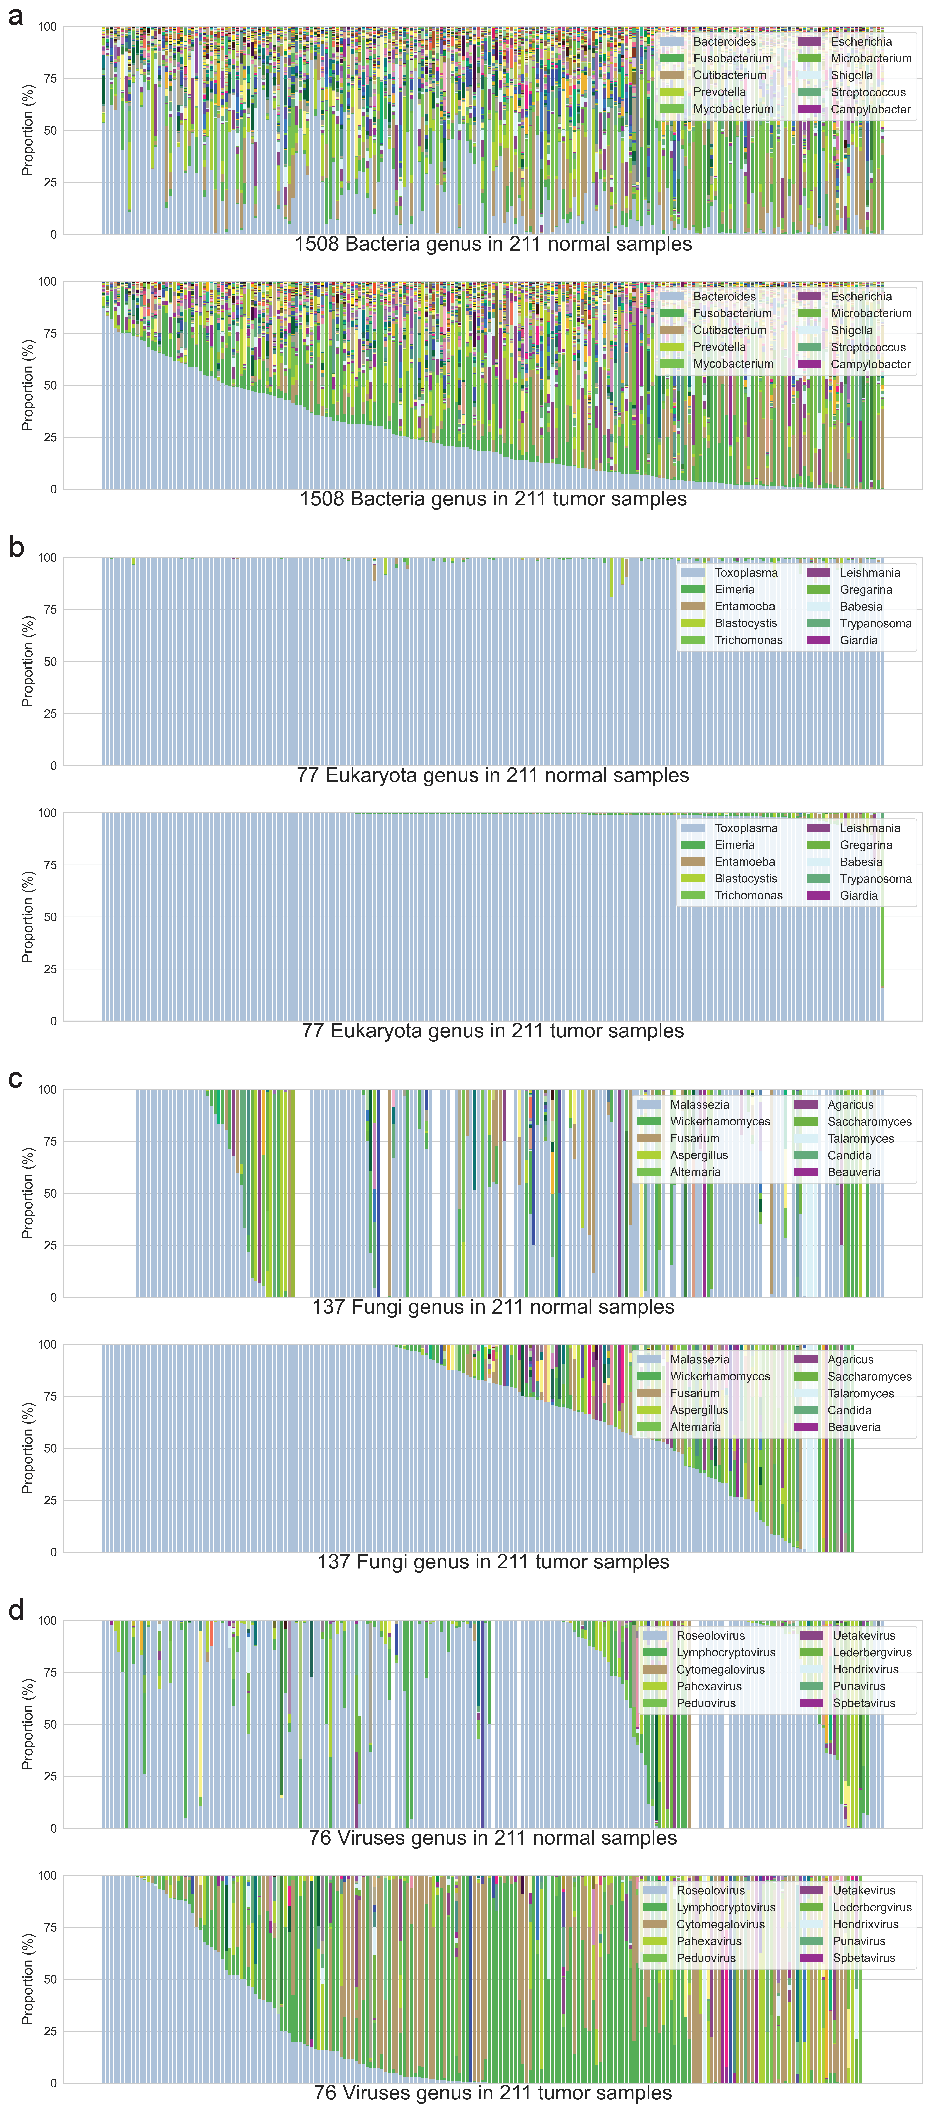
\includegraphics[width=\linewidth]{Figures/Periodontitis/Figure_1.pdf}
                \caption[Diversity indices]{\textbf{Diversity indices}. Comparisons of salivary microbiomes among healthy controls and patients with various periodontitis stages. Alpha-diversity indices \textbf{(a-e)} indicate that healthy controls have increased heterogeneity than periodontitis stages as measured by: \textbf{(a)} ace \textbf{(b)} chao1 \textbf{(c)} Fisher alpha \textbf{(d)} Margalef, and \textbf{(e)} observed ASVs. \textbf{(f)} The beta-diversity index (weighted UniFrac) was visualized using a tSNE-transformed plot. The confidence ellipses are shown to display the distribution of each periodontitis stage. The distance to each stage demonstrated that each periodontitis stage was distinguished from the other periodontitis stages: \textbf{(g)} distance to Healthy \textbf{(h)} distance to Stage I \textbf{(i)} distance to Stage II, and \textbf{(j)} distance to Stage III. Statistical significance determined by the Mann-Whitney U-test (MWU) test: $p \le 0.01$ (**) and $p \le 0.0001$ (****).}
                \label{fig:Periodontitis-diveristy}
            \end{figure}
            \clearpage

            \begin{figure}[p]
                \centering
                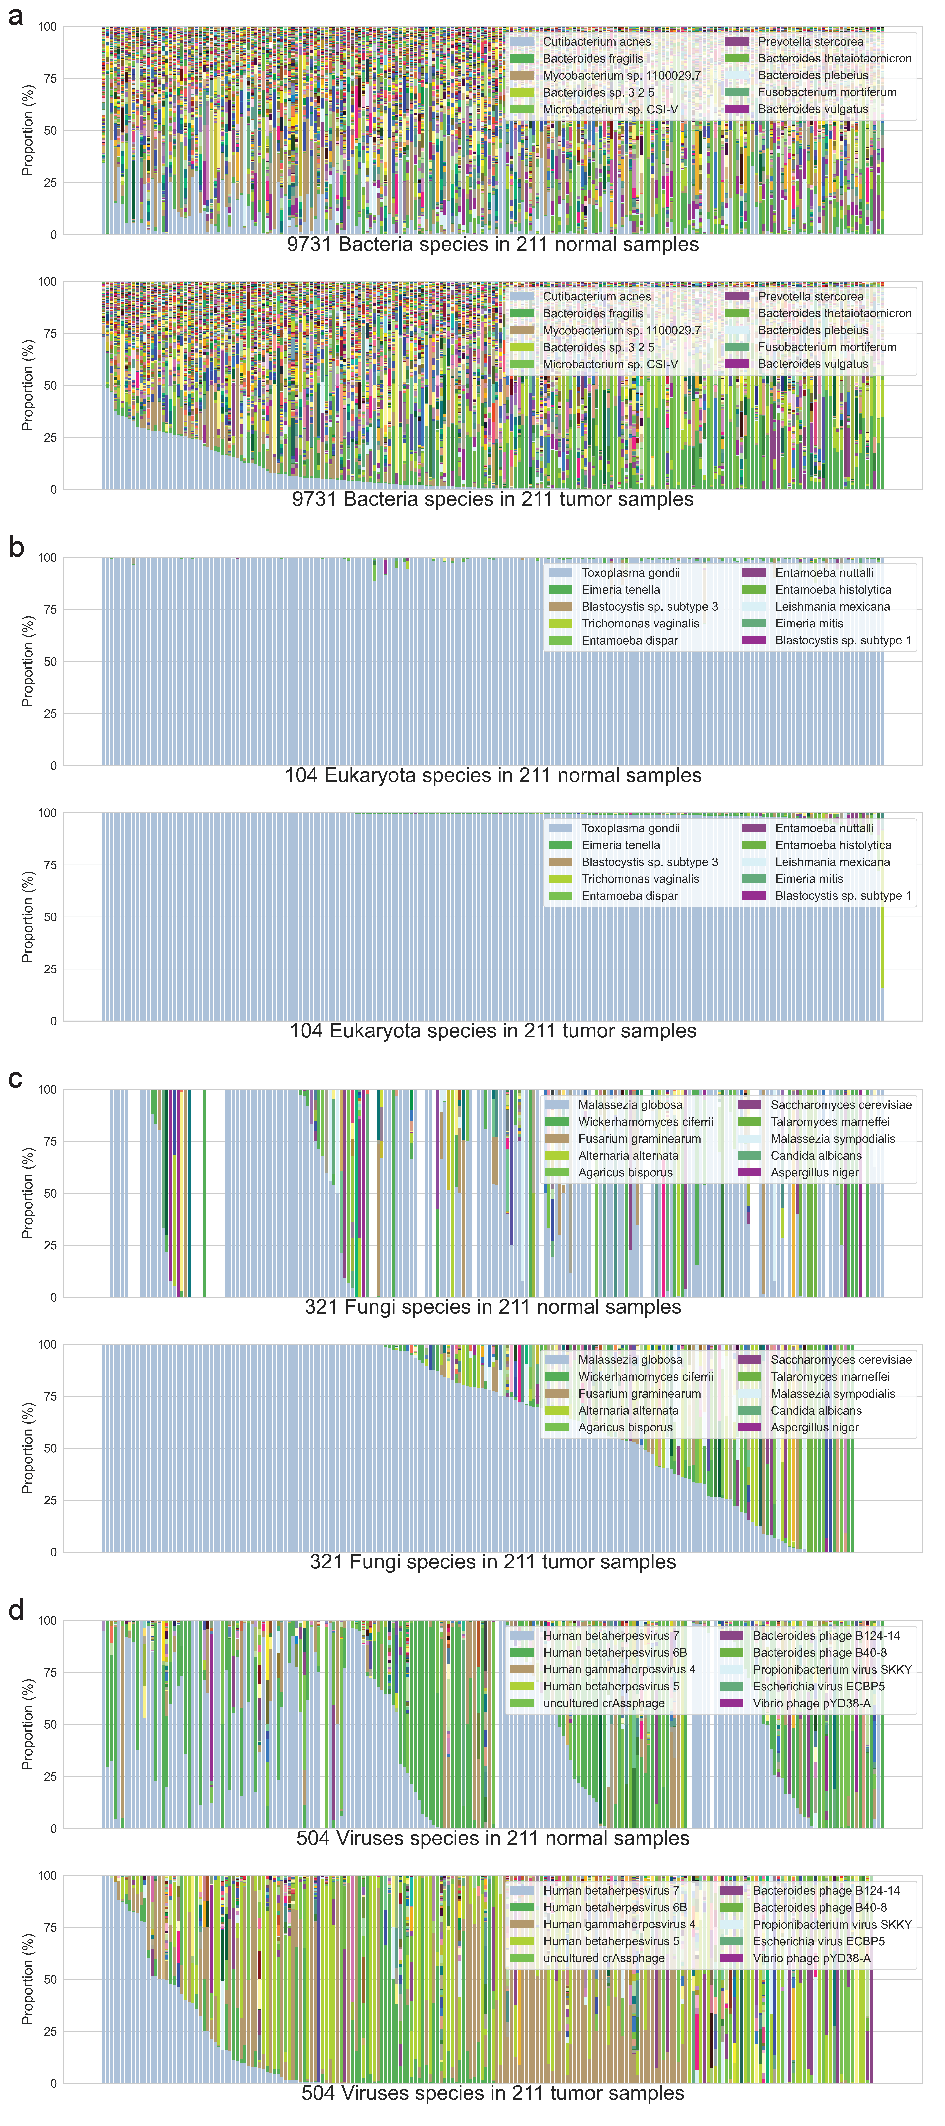
\includegraphics[width=\linewidth]{Figures/Periodontitis/Figure_2.pdf}
                \caption[Differentially abundant taxa]{\textbf{Differentially abundant taxa}. Differentially abundant taxa (DAT) that were identified by ANCOM. \textbf{(a)} Heatmap of clustered DAT with similar distribution among subjects. Group 1, Group 2, and Group 3 are marked in red, black, and green, respectively. \textbf{(b)} Box plots showing the proportions of DAT. Taxa were sorted by their importance according to ANCOM.}
                \label{fig:Periodontitis-DAT}
            \end{figure}
            \clearpage

            \begin{figure}[p]
                \centering
                \includegraphics[width=\linewidth]{Figures/Periodontitis/Figure_3.pdf}
                \caption[Correlation heatmap]{\textbf{Correlation heatmap}. Pearson’s correlations between differentially abundant taxa in healthy status and periodontitis stages. Statistical significance was determined by strong correlation, i.e., $| \textrm{coefficient} | \ge 0.5$ (*).}
                \label{fig:Periodontitis-correlation}
            \end{figure}
            \clearpage

            \begin{figure}[p]
                \centering
                \includegraphics[width=\linewidth]{Figures/Periodontitis/Figure_4.pdf}
                \caption[Random forest classification metrics]{\textbf{Random forest classification metrics}. The classification metrics in the random forest classifications were as follows: accuracy (ACC), area-under-curve (AUC), balanced accuracy (BA), F1 score (F1), precision (PRE), sensitivity (SEN), and specificity (SPE). Every classification metric ranges from [0, 1], with higher values indicating better performance. \textbf{(a)} Classification performance for healthy vs. stage I vs. stage II vs. stage III. \textbf{(b)} Receiver-operating characteristics (ROC) curve for the highest BA of (a). \textbf{(c)} Classification performance for healthy vs. stage I. \textbf{(d)} ROC curve on the highest BA of (c). (\textbf{e)} Classification performance for healthy vs. stage I vs. stages II/III. \textbf{(f)} ROC curve for the highest BA of (e). \textbf{(g)} Classification performance for healthy vs. stages I/II/III. \textbf{(h)} ROC curve for the highest BA of (h).}
                \label{fig:Periodontitis-ML}
            \end{figure}
            \clearpage

            \begin{figure}[p]
                \centering
                \includegraphics[width=\linewidth]{Figures/Periodontitis/Figure_5.pdf}
                \caption[Random forest classification metrics from external datasets]{\textbf{Random forest classification metrics from external datasets}. The classification metrics in the random forest classification included accuracy (ACC), balanced accuracy (BA), F1 score (F1), precision (PRE), sensitivity (SEN), and specificity (SPE). Every classification metric ranges from [0, 1], with higher values indicating better performance. (a) Classification performance for healthy vs. stage I vs. stage II vs. stage III. (b) Classification performance for healthy vs. stage I. (c) Classification performance for healthy vs. stage I vs. stages II/III. (d) Classification performance for healthy vs. stages I/II/III.}
                \label{fig:Periodontitis-validation}
            \end{figure}
            \clearpage

            \begin{figure}[p]
                \centering
                \includegraphics[width=0.75 \linewidth]{Figures/Periodontitis/Figure_S1.pdf}
                \caption[Rarefaction curves for alpha diversity indices]{\textbf{Rarefaction curves for alpha diversity indices}. Rarefaction of \textbf{(a)} chao1 \textbf{(b)} margalef, and \textbf{(c)} observed ASVs were generated to measure species richness and determine the sampling depth of each sample.}
                \label{fig:Periodontitis-rarefaction}
            \end{figure}
            \clearpage

            \begin{figure}[p]
                \centering
                \includegraphics[width=\linewidth]{Figures/Periodontitis/Figure_S2.pdf}
                \caption[Absolute abundance of salivary bacterial taxa in the different periodontal statuses at the species level]{\textbf{Absolute abundance of salivary bacterial taxa in the different periodontal statuses at the species level}. Stacked bar plot of the absolute abundance of bacterial species for all samples \textbf{(a)} and the mean absolute abundance of bacterial species in the healthy, stage I, stage II, and stage III groups \textbf{(b)}.}
                \label{fig:Periodontitis-abundance}
            \end{figure}
            \clearpage

            \begin{figure}[p]
                \centering
                \includegraphics[width=\linewidth]{Figures/Periodontitis/Figure_S3.pdf}
                \caption[Correlation plots for differentially abundant taxa]{\textbf{Correlation plots for differentially abundant taxa}. We selected the combinations of DAT with absolute Spearman correlation coefficients greater than 0.5. The color represents periodontal healthy periodontal statuses (green: healthy, cyan: stage I, yellow: stage II, and red: stage III).}
                \label{fig:Periodontitis-correlation2}
            \end{figure}
            \clearpage

            \begin{figure}[p]
                \centering
                \includegraphics[width=\linewidth]{Figures/Periodontitis/Figure_R02.pdf}
                \caption[Clinical measurements by the periodontitis statuses]{\textbf{Clinical measurements by the periodontitis statuses}. Comparisons of clinical measurement among healthy controls and patients with various periodontitis stages. (a) Clinical attachment level (b) Probing depth. Statistical significance determined by the Mann-Whitney U-test: p ≤ 0.01 (**) and p ≤ 0.0001 (****).}
                \label{fig:Periodontitis-clinical}
            \end{figure}
            \clearpage

            \begin{figure}[p]
                \centering
                \includegraphics[width=\linewidth]{Figures/Periodontitis/Figure_R03.pdf}
                \caption[Number of read counts by the periodontitis statuses]{\textbf{Number of read counts by the periodontitis statuses}. Comparisons of the number of read counts among healthy controls and patients with various periodontitis stages. (a) Before quality check (b) After quality check. Statistical significance determined by the Mann-Whitney U-test: p > 0.05 (ns), p ≤ 0.001 (***), and p ≤ 0.0001 (****).}
                \label{fig:Periodontitis-QC}
            \end{figure}
            \clearpage

            \begin{figure}[p]
                \centering
                \includegraphics[width=0.9 \linewidth]{Figures/Periodontitis/Figure_R04.pdf}
                \caption[Proportion of differentially abundant taxa]{\textbf{Proportion of differentially abundant taxa}. Proportions of differentially abundant taxa that were identified by ANCOM. (a) Actinomyces graevenitzii (b) Actinomyces spp. (c) Campylobacter showae (d) Corynebacterium durum (e) Filifactor alocis (f) Fretibacterium spp. (g) Lachnospiraceae [G-8] bacterium HMT 500 (h) Mycoplasma faucium (i) Peptostreptococcaceae [XI][G-5] saphenum (j) Peptostreptococcaceae [XI][G-6] nodatum (k) Peptostreptococcaceae [XI][G-9] brachy (l) Porphyromonas gingivalis (m) Porphyromonas sp. HMT 285 (n) Prevotella intermedia (o) Prevotella sp. HMT 304 (p) Prevotella sp. HMT 526 (q) Tannerella forsythia (r) Treponema putidum (s) Treponema sp. HMT 260 (t) Treponema spp. Statistical significance determined by the Mann-Whitney U-test: p > 0.05 (ns), p ≤ 0.05 (*), p ≤ 0.01 (**), p ≤ 0.001 (***), and p ≤ 0.0001 (****).}
                \label{fig:Periodontitis-proportions}
            \end{figure}
            \clearpage

            \begin{figure}[p]
                \centering
                \includegraphics[width=\linewidth]{Figures/Periodontitis/Figure_R05.pdf}
                \caption[Random forest classification metrics with the full microbiome compositions and ANCOM-selected DAT compositions]{\textbf{Random forest classification metrics with the full microbiome compositions and ANCOM-selected DAT compositions}. The classification metrics in the random forest classifications were as follows: accuracy (ACC), area-under-curve (AUC), balanced accuracy (BA), F1 score (F1), precision (PRE), sensitivity (SEN), and specificity (SPE). Every classification metric ranges from [0, 1], with higher values indicating better performance. (a) Classification performance for healthy vs. stage I vs. stage II vs. stage III. (b) Receiver-operating characteristics (ROC) curve for the highest BA of (a). (c) Classification performance for healthy vs. stage I. (d) ROC curve on the highest BA of (c). (e) Classification performance for healthy vs. stage I vs. stages II/III. (f) ROC curve for the highest BA of (e). (g) Classification performance for healthy vs. stages I/II/III. (h) ROC curve for the highest BA of (g). Statistical significance determined by the Mann-Whitney U-test test: p > 0.05 (ns), p ≤ 0.01 (**), and p ≤ 0.0001 (****).}
                \label{fig:Periodontitis-full}
            \end{figure}
            \clearpage

            \begin{figure}[p]
                \centering
                \includegraphics[width=\linewidth]{Figures/Periodontitis/Figure_R06.pdf}
                \caption[Alpha-diversity indices account for evenness]{\textbf{Alpha-diversity indices account for evenness}. Alpha-diversity indices (a-d) indicate that the heterogeneity between the periodontitis stages as measured by: (a) Berger-Parker d (b) Gini (c) Shannon (d) Simpson. Statistical significance determined by the Mann-Whitney U-test test: p ≤ 0.05 (*) and p ≤ 0.01 (**)}
                \label{fig:Periodontitis-alpha}
            \end{figure}
            \clearpage

            \begin{figure}[p]
                \centering
                \includegraphics[width=\linewidth]{Figures/Periodontitis/Figure_R09.pdf}
                \caption[Gradient Boosting classification metrics]{\textbf{Gradient Boosting classification metrics}. The classification metrics in the gradient boosting classifications were as follows: accuracy (ACC), area-under-curve (AUC), balanced accuracy (BA), F1 score (F1), precision (PRE), sensitivity (SEN), and specificity (SPE). Every classification metric ranges from [0, 1], with higher values indicating better performance. The feature counts mean that the classification model trained on the most important n features as the Supporting Table 2. (a) Comparison of Random forest (RF) and Gradient boosting (GB) for healthy vs. stage I vs. stage II vs. stage III. (b) Comparison of RF and GB for the highest BA of (a). (c) Classification performance for healthy vs. stage I. (d) Comparison of RF and GB for healthy vs. stage I vs. stages II/III. (f) Comparison of RF and GB for Healthy vs. Stage I vs. Stages II/III. (g) Classification performance for healthy vs. stages I/II/III. (h) Comparison of RF and GB for Healthy vs. Stages I/II/III.}
                \label{fig:Periodontitis-GB}
            \end{figure}
            \clearpage
        \newpage

        \subsection{Discussion}
        \newpage

    \section{Lung microbiome}
        \subsection{Introduction}
        \clearpage

        \subsection{Materials and methods}
        \clearpage

        \subsection{Results}
        \clearpage

        \subsubsection{Discussion}
        \clearpage
    \newpage

    \section{General conclusion and future perspective}
        \label{section:conclusion}
        \subsection{General conclusions}
            In conclusion, the research described in this doctoral dissertation was conducted to identify significant ...

            In the Section \ref{section:PTB}, I show that
        \newpage

        \subsection{Plan for future}
        \newpage

        \subsection{Future perspective}
        \newpage

% Reference
    \addcontentsline{toc}{section}{References}
    \bibliographystyle{apacite}
    \bibliography{references.bib}
    \clearpage

% Acknowledgements
    \addcontentsline{toc}{section}{Acknowledgments}
    \section*{\hfill \Large Acknowledgments \hfill}
        I would like to disclose my earnest appreciation for my advisor, Professor Semin Lee, who provided solicitous supervision and cherished opportunities throughout the course of my research. His advice and consultation encouraged me to become as a researcher and to receive all humility and gentleness. I am also grateful to all of my committee members, Professor AAA, Professor BBB, Professor CCC, and Professor DDD, for their critical and meaningful mentions and suggestions.

        I extend my deepest gratitude to my Lord, \textit{the Flying Spaghetti Monster}, His Noodly Appendage has guided me through the twist and turns of this academic journey. His presence, ever comforting and mysterious, has been a source of strength and humor during both highs and lows. In moments of doubt, I found solace in the belief that you were there, gently reminding me to keep faith in the process. His Holy Noodle has nourished my mind, and for that, I am truly overwhelmed. May His Holy Noodle continue to guide me in all my future endeavors. R'Amen.

        (Professors)

        I would like to extend my heartfelt gratitude to my colleagues of the Computational Biology Lab @ UNIST, whose collaboration, friendship, brotherhood, and support have been an invaluable part of my journey. Your willingness to share insights, engage in thoughtful discussions, and offer encouragement during the challenging moments of research has significantly shaped my academic experience. The camaraderie in Computational Biology Lab made even the most demanding days more enjoyable, and I am deeply grateful for the collaborative environment we created together. I appreciate you for standing by my side throughout this Ph.D. journey.

        I would like to express my heartfelt gratitude to my family, whose unwavering support has been the foundation of everything I have achieved. Your love, encouragement, and belief in me have sustained me through every challenge, and I could not have come this far without you. From your words of wisdom to your patience and understanding, each of you has played a vital role in helping me navigate this journey. The strength and comfort I have drawn from our family bond have been my greatest source of resilience. Your presence, both near and far, has filled my life with warmth and motivation. I am deeply grateful for your unconditional love and for always being there when I needed you the most. Thank you for being my constant source of strength and inspiration.

        I am incredibly pleased to my friends, especially my GSHS alumni (이망톡), for their unwavering support and encouragement throughout this journey. The bonds we formed back in our school days have only grown stronger over the years, and I am fortunate to have had such loyal and understanding friends by my side. Your constant words of motivation, and even moments of levity during stressful times have helped keep me grounded. Whether it was a late-night conversations, a shared laugh, or a simple message of reassurance, you all have played a vital role in keeping me focused and motivated. I am relieved for the ways you celebrated each small achievement with me and how you patiently listened to my worries. The memories of our shared past provided me with comfort and a sense of stability when the road ahead felt uncertain. I could not have reached this point without the love and friendship that you all have generously given. Each of your, in your unique way, has contributed to this dissertation, even if indirectly, and for that, I am forever beholden. I look forward to continuing our friendship as we all grow in our individual paths, knowing that the support we share is something truly special.

        I would like to express my sincere gratitude to the amazing members of my animal protection groups, DRDR (두루두루) and UNIMALS (유니멀스), whose dedication and compassion have been a constant source of motivation. Your unwavering commitment to improving the lives of animals has inspired me throughout this journey. I am also thankful for the beautiful cats we have cared for, whose presence brought both joy and purpose to our allegiance. Their playful spirits and gentle companionship served as daily reminders of why we continue to fight for animal rights. The bond we share, both with each other and with the animals we protect, has enriched my life in countless ways. I appreciate you all again for your support, dedication, and for being part of this meaningful cause.

        I would like to express my deepest gratitude to everyone I have had the honor of meeting throughout this journey. Your kindness, encouragement, and support have carried me through both the challenging and rewarding moments of my life. Whether through a kind word, thoughtful advice, or simply being there when I needed it most, your presence has made all the difference. I am incredibly fortunate to have received such generosity and warmth from those around me, and I do not take it for granted. Every act of kindness, no matter how big or small, has been a source of strength and motivation for me. To all my friends, colleagues, mentors, and beloved ones, thank you for your unwavering support. I am truly grateful for each of you, and your kindness has left an indelible mark on my journey.

        \begin{center}
            My Lord, \textit{the Flying Spaghetti Monster},\\
            give us grace to accept with serenity the things that cannot be changed,\\
            courage to change the things that should be changed,\\
            and the wisdom to distinguish the one from the other.

            \medspace

            Glory be to \textit{the Meatball}, to \textit{the Sauce}, and to \textit{the Holy Noodle}. \\
            As it was in the beginning, is now, and ever shall be. \\
            R'Amen.
        \end{center}
    \clearpage

%%% The following page is intentionally left as blank
% White attachment form
\hbox{ }
\thispagestyle{empty}
\clearpage
\end{document}